\chapter*{BIODATA PENULIS}
%*********************************
%Gambar Foto 
	\begin{center}
		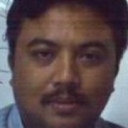
\includegraphics[height=0.2\textheight]{./ubah/Foto}
	\end{center}
%*********************************
\section*{Identitas Diri}
\begin{tabular}{p{3cm}cp{9cm}}
	%Masukan Identitas Disini.............
	Nama  		  & :&
		Eko Mulyanto Yuniarno \\
	Tempat Lahir  & :&
		Surabaya\\
	Tanggal Lahir &:& 
		12 Desember 2021\\
	Alamat        &:& J
		alan Jati No 4,Kampung Hutan, Kecamatan Danau, Kabupaten Siak\\
	Identitas 1   &:&
		 Isi Identitas 1\\
	Identitas 2   &:& 
		Isi Identitas 2\\
	Identitas 3   &:&
		 Isi Identitas 3\\
	Identitas 4   &:&
		 Isi Identitas 4\\
\end{tabular}

\section*{Riwayat Pendidikan}
\begin{tabular}{p{3cm}cp{9cm}}
	2019-Sekarang  	& :&
		Program Doktor (S3), Departemen Teknik  Elektro, Fakultas Teknologi Elektro dan Informatika Cerdas, Institut Teknologi  Sepuluh Nopember\\
	&&\\
	2014-2019  & :&
		Program Master (S2), Departemen Teknik  Elektro, Fakultas Teknologi Elektro dan Informatika Cerdas, Institut Teknologi  Sepuluh Nopember\\
	&&\\
	2011-2014  & :&
		Program Sarjana (S1), Departemen Teknik  Elektro, Fakultas Teknologi Elektro dan Informatika Cerdas, Institut Teknologi  Sepuluh Nopember\\
	&&\\
	0000-0000  & :&
		Pendidikan 1\\
	&&\\
	0000-0000  & :&
		Pendidikan 2\\
	&&\\
	0000-0000  & :&
		Pendidikan 3\\
\end{tabular}


\section*{Daftar Publikasi}

\begin{enumerate}
	\item Setiyoutami, A., Anggraeni, W., Purwitasari, D., Yuniarno, E.M., Purnomo, M.H.,\textit{Extracting Temporal-Based Spatial Features in Imbalanced Data for Predicting Dengue Virus Transmission},
	Advances in Intelligent Systems and Computing, 2021, 1158, pp. 731–742
	\item Salsabila, F.N., Yuhana, U.L., Yuniarno, E.M., Purnomo, M.H., \textit{Sifte-math, a sifteo based mathematics assessment serious game for deaf children}, IES 2020 - International Electronics Symposium: The Role of Autonomous and Intelligent Systems for Human Life and Comfort, 2020, pp. 620–625, 9231578
	
	
\end{enumerate}

\section*{Riwayat Penelitian}
\begin{enumerate}
	\item \lipsum[3]
	\item \lipsum[3]
	\item Penelitian Ke Tiga 
	\item Penelitian Ke Empat 
\end{enumerate}
\section*{Riwayat Lainnya}

\lipsum[1]